\section{Failure Modes of Shafts}

\newthought{There are a number of shaft failure modes} and it is important to recognise the types of failure that can occur and be able to perform the subsequent analysis to mitigate this occurring within our design. It is up to you to do some research on the types of failure and to discuss the failures that might occur for your shaft. Whilst this section does not detail the types of failure, it does provide the calculations required to determine the stresses within the shaft so that you will be able to evaluate whether the shaft will survive the forces that it is being subjected to.

\subsection{Types of Failure}

\begin{framed}
  \vspace{0.5cm}
    \begin{center}
      {\fontsize{50}{60}\selectfont ?}\\
      Own Research \& Lectures
    \end{center}
  \vspace{0.5cm}
\end{framed}

%\marginnote{\it overloading}

%\marginnote{\it fatigue}

%\marginnote{\it torsional fatigue}

%\marginnote{\it rotational loading}

\subsection{Calculating Shaft Stresses}

\marginnote{Direct Stress $(\sigma_d)$} The first is the direct stress acting through the cross-section of the shaft. If the shaft diameter is not large enough then shaft will simply shear as if one were creating a cross-section through the shaft. The Direct Stress is given by Equation~\ref{equ-direct-stress}.

\begin{equation}
  \sigma_d = \frac{F}{A}
  \label{equ-direct-stress}
\end{equation}

However, it is very rare for a shaft to fail through Direct Stress through the shafts cross-section. It is more likely that a shaft will fail due to the combined bending, hoop and torsional stresses acting on the outer surface of the shaft, which can be resolved using Mohr's Circle~\cite{clifford2012}.

Taking\marginnote{Mohr's circle}  a 2D element on the outer surface of the shaft, the bending, hoop and torsional stresses can be related as shown in \cref{fig-mohrs-circle}. Where $\sigma_x$ is the bending stress, $\sigma_y$ is the hoop stress and $\tau_{xy}$ is the torsional stress.

\begin{marginfigure}
  \center{}
  \begin{tikzpicture}[scale=2]

    \draw[] (0,0) -- (0,1) -- (1,1) -- (1,0) -- (0,0);


    \draw[->] (-0.1,0.5) -- (-0.4,0.5) node[left]{$\sigma_x$};
    \draw[->] (1.1,0.5) -- (1.4,0.5) node[right]{$\sigma_x$};
    \draw[->] (0.5,1.1) -- (0.5,1.4) node[above]{$\sigma_y$};
    \draw[->] (0.5,-0.1) -- (0.5,-0.4) node[below]{$\sigma_y$};

    \draw[{Straight Barb[left]}-] (0.0,-0.05) -- (1.0,-0.05) node[pos=0.0, below]{$\tau_{xy}$};
    \draw[-{Straight Barb[left]}] (0.0,1.05) -- (1.0,1.05) node[pos=1.0, above]{$\tau_{xy}$};

    \draw[{Straight Barb[right]}-] (-0.05,0.0) -- (-0.05,1.0) node[pos=0.0, left]{$\tau_{xy}$};
    \draw[-{Straight Barb[right]}] (1.05,0.0) -- (1.05,1.0) node[pos=1.0, right]{$\tau_{xy}$};

  \end{tikzpicture}
  \caption{2D mohr's circle}
  \label{fig-mohrs-circle}
\end{marginfigure}

Bending\marginnote{Bending Stress $(\sigma_x)$}  stress is the Direct Stress in the direction of the axis of the shaft and is due to the bending moment. This can be calculated using Equation~\ref{equ-bending-stress}.

\begin{equation}
  \sigma_{x} = \frac{My}{I}
  \label{equ-bending-stress}
\end{equation}

Where \(I\) is the Second Moment of Area:

\begin{equation}
  I = \frac{\pi r^4}{4}
\end{equation}

Hoop\marginnote{Hoop Stress \(\sigma_y\)} stress is the direct stress due to forces attempting to expand the shaft. This is only really the case when considering pressure vessels where the interior pressure of the gas or liquid is wanting to expand the vessel. In our cases, we can say that \(\sigma_y = 0\). 

Torsional\marginnote{Torsional Stress \(\tau_{xy}\)} stress is the shear stress due to torsion (twisting) and can by calculated using Equation~(\ref{equ:torsional-stress}).

\begin{equation}
  \tau_{xy} = \frac{Tr}{J}
  \label{equ:torsional-stress}
\end{equation}

Where \(J\) is the Polar Moment of Area:

\begin{equation}
  J = \frac{\pi d^4}{32}
\end{equation}

These stress depend upon the orientation of the element. If another element is taken, twisted through an angle \(\phi\), as shown in Figure, then the Direct Stresses are \(\sigma_x\) and \(\sigma_X\) and the shear stress is \(\tau_{xy}\) = \(\tau_{XY}\). And these are normally different from the first set of stresses in \cref{fig-rotated-mohrs-circle}.

\begin{marginfigure}
  \center{}
  \begin{tikzpicture}[scale=2]

    \draw[rotate=45] (0,0) -- (0,1) -- (1,1) -- (1,0) -- (0,0);


    \draw[->, rotate=45] (-0.1,0.5) -- (-0.4,0.5) node[left]{$\sigma_X$};
    \draw[->, rotate=45] (1.1,0.5) -- (1.4,0.5) node[right]{$\sigma_X$};
    \draw[->, rotate=45] (0.5,1.1) -- (0.5,1.4) node[above]{$\sigma_Y$};
    \draw[->, rotate=45] (0.5,-0.1) -- (0.5,-0.4) node[below]{$\sigma_Y$};

    \draw[{Straight Barb[left]}-, rotate=45] (0.0,-0.05) -- (1.0,-0.05) node[pos=0.0, below]{$\tau_{XY}$};
    \draw[-{Straight Barb[left]}, rotate=45] (0.0,1.05) -- (1.0,1.05) node[pos=1.0, above]{$\tau_{XY}$};

    \draw[{Straight Barb[right]}-, rotate=45] (-0.05,0.0) -- (-0.05,1.0) node[pos=0.0, left]{$\tau_{XY}$};
    \draw[-{Straight Barb[right]}, rotate=45] (1.05,0.0) -- (1.05,1.0) node[pos=1.0, right]{$\tau_{XY}$};

  \end{tikzpicture}
  \caption{Mohr's circle rotated by \(\phi\)}
  \label{fig-rotated-mohrs-circle}
\end{marginfigure}

The two sets of stresses are related by formulae involving the sine and cosine of twice the angle, 2\(\phi\). Mohr's circle is a graphical way of representing these formulae. The construction of the circle is as follows and is shown in \cref{fig-m-circle}.

\begin{enumerate}
  \item Draw the line AB between points with coordinates: \(\text{A} = (\sigma_x, -\tau_{xy}) \) and \(\text{B} = (\sigma_y, \tau_{xy}) \)
  \item Draw the circle with AB as diameter
\end{enumerate}



\begin{figure}[h!]
  \center{}
  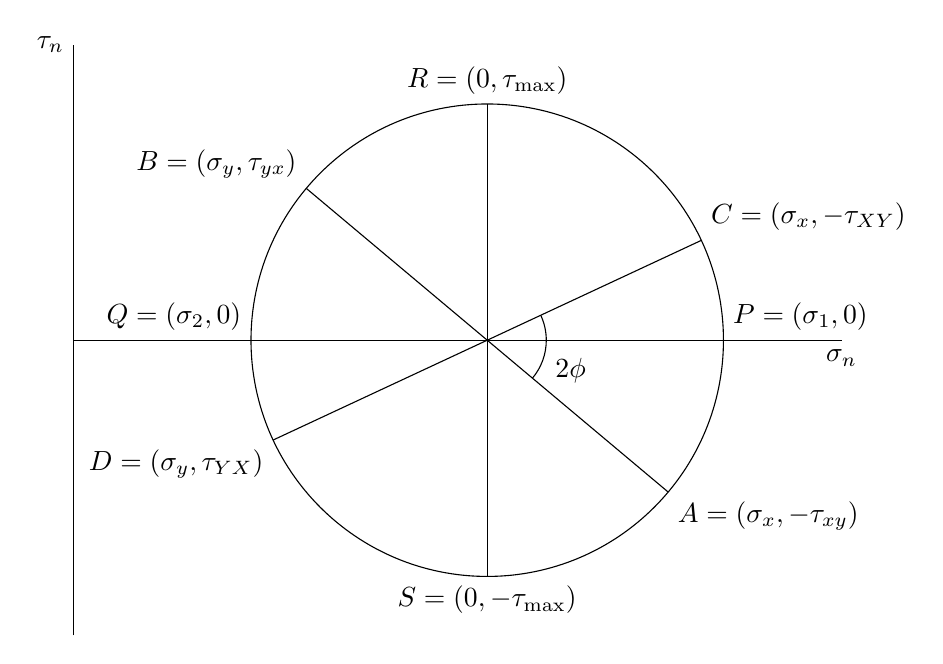
\begin{tikzpicture}[scale=0.75]

    \draw[] (-1,-5) -- (-1,5) node[pos=1.0, anchor=east] {$\tau_n$};
    \draw[] (-1,0) -- (12,0) node[pos=1.0, anchor=north] {$\sigma_n$};
  
    \draw[] (6,0) circle (4);
  
    \draw[] (2,0) -- (10,0)
    node[pos=0.0, anchor=south east] {$Q=(\sigma_2,0)$}
    node[pos=1.0, anchor=south west] {$P=(\sigma_1,0)$};
  
    \draw[] (6,-4) -- (6,4)
    node[pos=0.0, anchor=north] {$S=(0,-\tau_{\max} )$}
    node[pos=1.0, anchor=south] {$R=(0,\tau_{\max} )$};
  
    \draw[rotate around={25:(6,0)}] (2,0) -- (10,0) 
    node[pos=0.0, anchor=north east] {$D=(\sigma_y,\tau_{YX})$}
    node[pos=1.0, anchor=south west] {$C=(\sigma_x,-\tau_{XY})$};
  
    \draw[rotate around={-40:(6,0)}] (2,0) -- (10,0) 
    node[pos=0.0, anchor=south east] {$B=(\sigma_y,\tau_{yx})$}
    node[pos=1.0, anchor=north west] {$A=(\sigma_x,-\tau_{xy})$};
  
    \draw[] (7,0) arc (0:25:1);
    \draw[] (7,0) arc (0:-40:1) node[pos=0.2, anchor=north west] {$2\phi$};
  
  \end{tikzpicture}
  \caption{Mohr's circle relating stresses associated with elements with different orientations}
  \label{fig-m-circle}
\end{figure}

Then, to find the stresses related to the element rotated through angle \(\phi\), the diameter AB is rotated through angle \(2\phi\), giving diameter CD. The positions of C and D give the other stress with: \(\text{C} = (\sigma_X, -\tau_{XY}) \) and \(\text{D} = (\sigma_Y, \tau_{XY}) \).

Mohr's\marginnote{Principal Stresses} circle shows there are two special cases. The first is when the diameter AB is rotated so that it becomes horizontal. The corresponding element undergoes no shear stress, but is subject to two direct stresses (in perpendicular directions) which are \(\sigma_1\) and \(\sigma_2\). These are the principal direct stress and represent the maximum and minimum values of direct stress in any direction.

\begin{equation}
  \sigma_1 = \frac{1}{2}(\sigma_x+\sigma_y) + \sqrt{\left(\frac{1}{4}(\sigma_x-\sigma_y)^2\right)+\tau_{xy}^2}
\end{equation}

\begin{equation}
  \sigma_2 = \frac{1}{2}(\sigma_x+\sigma_y) - \sqrt{\left(\frac{1}{4}(\sigma_x-\sigma_y)^2\right)+\tau_{xy}^2}
\end{equation}

The\marginnote{Principal Shear Stresses} second special case is when the diameter AB is rotated so that it becomes vertical in circle. The corresponding element sees the same direct stresses (in the two perpendicular directions) and a shear stress. From \cref{fig-m-circle}, this common direct stress is the average of the principal stresses \(\frac{1}{2}(\sigma_1+\sigma_2)\). The shear stress is the largest possible shear stress in any direction, denoted (on \cref{fig-m-circle}) by \(\tau_{\max}\).

\begin{equation}
  \tau_{\max} = \sqrt{\left(\frac{1}{4}(\sigma_x-\sigma_y)^2\right)+\tau_{xy}^2}
  \label{equ:tau-max}
\end{equation}

In designing a component, there are limiting values placed on the direct and shear stresses (associated with any elements or directions). These may be based upon the yield tensile stress and the yield shear stress, or upon the ultimate tensile stress and ultimate shear stress.

So there are two conditions to satisfy as follows.

\begin{equation}
|\sigma_1|,|\sigma_2| \leq \text{max\ allowable\ direct\ stress}
\end{equation}

\begin{equation}
|\tau_{\max}| \leq \text{max\ allowable\ shear\ stress}
\end{equation}

The\marginnote{Assumptions for Shafts} first assumption is that only stresses on the outside of the shaft need be considered. This is where the axial direct stress and the shear stress are maximal.

The second assumption is that only the condition related to the maximum shear stress needs to be considered. This is because of the observation that shafts made of ductile materials tend to fail due to shear.

The third assumption is that the \acf{UTS} and the \acf{USS} for steel and roughly related by the relation:

\begin{equation}
  \text{USS steel} \simeq 0.75 \times \text{UTS steel}
\end{equation}

An alternative third assumption is that the \acf{TYS} and the \acf{SYS} for steel are roughly related by the relation:

\begin{equation}
  \text{SYS steel} \simeq 0.58 \times \text{TYS steel}
\end{equation}

These are empirical relations based upon typical values for steel as shown in \cref{tbl-uts-relationships} by~\citet{deutschman1975}~\cite{deutschman1975}.

\begin{table}
  \caption[Approximate relationships between shear and tensile stresses]{Approximate relationships between shear and tensile stresses~\citep{deutschman1975}}
  \label{tbl-uts-relationships}
  \center{}
  \small
  \begin{tabular}{p{0.2\textwidth} p{0.35\textwidth} p{0.35\textwidth}}
    \toprule
    Material & Ultimate strength relationship & Yield strength relationship \\
    \midrule
    steels & \(\text{USS } \simeq 0.75 \times \text{UTS}\) & \(\text{SYS} \simeq 0.58 \times \text{TYS}\) \\
    ductile iron & \(\text{USS } \simeq 0.9 \times \text{UTS}\) & \(\text{SYS} \simeq 0.75 \times \text{TYS}\) \\
    malleable iron & \(\text{USS } \simeq 1.0 \times \text{UTS}\) &  \\
    wrought iron & \(\text{USS } \simeq 0.83 \times \text{UTS}\) &  \\
    cast iron & \(\text{USS } \simeq 1.3 \times \text{UTS}\) &  \\
    aluminiums & \(\text{USS } \simeq 0.65 \times \text{UTS}\) & \(\text{SYS} \simeq 0.55 \times \text{TYS}\) \\
    \bottomrule
  \end{tabular}
\end{table}

\section{Failure Criteria}

The\marginnote{Note: to deal with these theories properly requires considering the stress in the third dimension, which we have been ignoring as it is zero for the cases considered here. While the failure criteria are completely general, to keep things simple the equations in this section are not necessarily valid for other general stress states.} yield strength of materials is measured experimentally, often using uniaxial tests. In this type of test, a sample is progressively loaded in tension, and its extension recorded, until it starts to deform plastically. The stress at this point is called the yield strength of the material. However, the combined stress state described above is more complicated than in a uniaxial test. It is not feasible to experimentally test for every combination of stresses that a material might encounter, so some theory is needed to relate the combined stress state described above to the uniaxial yield strength of the material. There are multiple theories available to explain this relationship, known as failure criteria. Here we will discuss the two simplest, the Tresca criteria and the von Mises stress.

The Tresca criterion is based on the maximum shear stress, and predicts that failure will occur when the maximum shear stress reaches some critical value:

\begin{equation}
  \tau_{\max} = \tau_{\text{failure}}
\end{equation}

The Tresca\marginnote{Tresca criterion} criterion is based on the maximum shear
stress, and predicts that failure will occur when the maximum shear stress
reaches some critical value:

\begin{equation}
\label{eq:2}
\tau_\mathrm{max} = \tau_\mathrm{failure}
\end{equation}

The critical value is calibrated to the yield strength $S_y$ measured in a
uniaxial test. In the uniaxial test at the onset of yield, $\sigma_x = S_y$ and
$\sigma_y = \tau_{xy} = 0$. From \cref{equ:tau-max},

\begin{equation}
\label{eq:4}
\tau_\mathrm{failure} = \sqrt{\left(\frac{\sigma_x-\sigma_y}{2}\right)^2+\tau_{xy}^2} = \sqrt{\left(\frac{S_y-0}{2}\right)^2+0} = \frac{S_y}{2}
\end{equation}

Therefore, the Tresca failure criterion (\cref{eq:2}) for shafts under bending
and torsion (\cref{equ:tau-max}) can be written as:

\begin{align}
\label{eq:5}
\frac{1}{2} \sqrt{\sigma_x^2+4\tau_{xy}^2} &= \frac{S_y}{2} \\
              \intertext{or simply}
  \label{eq:tresca-failure}
\sqrt{\sigma_x^2+4\tau_{xy}^2} &= S_y
\end{align}

The von Mises\marginnote{von Mises criterion} criterion is an alternative
theory. It has the advantage of being more accurate than the Tresca criterion
(which is always more conservative) and behaves in a more continuous manner when
the stress state is varying. The `von Mises stress' is defined as

\begin{equation}
\label{eq:7}
\sigma' = \left[ \frac{ 
    \left( \sigma_1 - \sigma_2 \right)^2 +
    \left( \sigma_2 - \sigma_3 \right)^2 +
    \left( \sigma_3 - \sigma_1 \right)^2
  }{2} \right]^{1/2}
\end{equation}

Here $\sigma_3$ is the principle stress in the third dimension, which can be
assumed to be zero for the shaft stresses we are considering here. The
expression can be simplified then to:

\begin{align}
\label{eq:9}
  \sigma' &= \left[ \frac{ 
  \left( \sigma_1 - \sigma_2 \right)^2 + \sigma_2^2 + \sigma_1^2
  }{2} \right]^{1/2} \\
&= \left[ \frac{\left( \sigma_1^2 + \sigma_2^2 - 2 \sigma_1\sigma_2 \right) + \sigma_2^2 + \sigma_1^2}{2} \right]^{1/2} \\
          &= \left[ \sigma_1^2 + \sigma_2^2 - \sigma_1\sigma_2 \right]^{1/2} 
\end{align}

Substituting for $\sigma_1$ and $\sigma_2$ from \cref{equ:tau-max}, this can be written
as:

\begin{align}
\sigma' &= \frac{1}{2} \left[
          \left( \sigma_x + \sqrt{\sigma_x^2+4\tau_{xy}^2} \right)^2 +
          \left( \sigma_x - \sqrt{\sigma_x^2+4\tau_{xy}^2} \right)^2 -
          \left( \sigma_x + \sqrt{\sigma_x^2+4\tau_{xy}^2} \right)
          \left( \sigma_x - \sqrt{\sigma_x^2+4\tau_{xy}^2} \right)
          \right]^{1/2} \\
&= \frac{1}{2} \left[\sigma_x^2 + 3\left( \sigma_x^2+4\tau_{xy}^2 \right) \right]^{1/2} \\
  &= \sqrt{\sigma_x^2 + 3\tau_{xy}^2}
  \label{eq:8}
\end{align}

The von Mises failure criterion for a shaft under bending and torsion is
therefore:

\begin{equation}
\sqrt{\sigma_x^2 + 3\tau_{xy}^2} = S_y
\label{eq:10}
\end{equation}

Comparing this to \cref{eq:5}, you might be able to see that the Tresca
criterion will always predict failure at the same or lower stress than the von
Mises criterion. In the end, it is no more complicated to use \cref{eq:10} than
\cref{eq:5}, so the von Mises criterion is often a good approach to use.